\section{Reproducibility and additional numerical results}\label{app:numerics}

\subsection{Simulation generating mechanism}\label{app:simulation-design}

The factorial design uses $n\in\{200,400\}$ subjects and $m\in\{5,20,80\}$ observations per subject, with 1,000 datasets in each configuration. All observation times are independent Uniform$(0,1)$. Set $b(t)=(1,\sin(2\pi t),\cos(2\pi t))^\trans$ and define
\[
\bX_i(t)=\{1,A_{i1}^\trans b(t)/\sqrt2,\ldots,
A_{i,p-1}^\trans b(t)/\sqrt2\}^\trans,
\]
where all entries of the $A_{ik}$ are independent standard normals. Independently, generate
\[
\varepsilon_i(t)=Z_{i0}+\tfrac12Z_{i1}\sin(2\pi t)
+\tfrac12Z_{i2}\cos(2\pi t).
\]
The $Z$ variables are independent draws from one of three laws: $N(0,1)$, Laplace$(0,1/\sqrt2)$, or $(\chi^2_5-5)/\sqrt{10}$. Here the Laplace parameter is its scale; the chi-square law is centered and standardized by its mean 5 and standard deviation $\sqrt{10}$. All three have mean zero, variance one, and finite moments of every fixed order. Responses are generated as $Y_{ij}=\bX_i(T_{ij})^\trans\bbeta(T_{ij})+\varepsilon_i(T_{ij})$, using this single functional error. Thus $\bOmega(t)=\bI_p$ and $\bC(t,t)=1.25\bI_p$ for every law.

For $p=2$, take $\beta_1(t)=0.5+0.5t$ and $\beta_2(t)=0.5+0.4\sin\{2\pi(t-0.5)\}$, and target $\beta_2$. For $p=5$, add $\beta_3(t)=0.3\cos(2\pi t)$, $\beta_4(t)=0.5t^2$, and $\beta_5(t)=0.4e^{t-1}$, and target all five functions jointly. The intercept-only mean comparison uses the same error process and the mean curve specified below. Local linear fits use the Epanechnikov kernel and $B=1{,}999$ Gaussian multiplier draws. All comparisons evaluate coverage and width on the same 201 equally spaced points in $[0.15,0.85]$.

\subsection{Computation and comparator formulas}\label{app:comparator-formulas}

Epanechnikov-weighted local moments are evaluated by exact polynomial prefix sums. Observation times are not binned, and residuals are fitted at every actual observation time, throughout the observation domain. Local Gram eigenvalues and variance positivity are checked; no ridge term or silent regularization is applied. A failed fit is counted as noncoverage. All methods within a comparison use the same dataset and target event.

The simulation bandwidth is \eqref{eq:local-linear-phase-bandwidth}, with multiplicative constant one. It is determined by $n$ and the counts, without using observed coverage or responses. The estimate, residuals, and multiplier covariance use that common value. This is a controlled comparison at specified tuning parameters, not a claim about the relative performance of all possible tuning rules.

For CLZ, put $N=\sum_i m_i$ and use the pooled local linear fit and its residuals. We use the same estimation bandwidth for both methods and for all nuisance kernel estimates; the original CLZ cross-validation choices are not imposed on either estimator. With equal counts and this common bandwidth, the two point estimates agree. Following equations (3.2), (3.5), and (3.6) of \citet{cao_simultaneous_2018}, compute
\begin{align*}
\widehat f(t)&=N^{-1}\sum_{ij}K_h(T_{ij}-t),\\
\widehat\Omega(t)&=N^{-1}\sum_{ij}K_h(T_{ij}-t)\bX_{ij}\bX_{ij}^\trans,\\
\widehat\Lambda(t)&=N^{-1}\sum_{ij}K_h(T_{ij}-t)\bX_{ij}\bX_{ij}^\trans\widehat\varepsilon_{ij}^{\,2}.
\end{align*}
The pointwise standard error for coefficient $k$ is
\[
\left[\frac{\nu_K}{Nh\widehat f(t)}
\{\widehat\Omega(t)^{-1}\widehat\Lambda(t)\widehat\Omega(t)^{-1}\}_{kk}\right]^{1/2},
\qquad \nu_K=\int K^2=3/5.
\]
These formulas reproduce the stated raw kernel-moment normalization for the uniform-design experiments. They are not presented as density-normalized conditional-moment estimates for an arbitrary nonuniform design. The normalization uses the total observation count $N$, not the number of subjects.

Their Section 3 critical-value simulation generates fresh independent $U_1,\ldots,U_N\sim\mathrm{Uniform}(0,1)$ and $g_1,\ldots,g_N\sim N(0,1)$, and records
\[
\max_{t\in\mathcal G}
\frac{\left|\sum_{a=1}^N g_a K\{(U_a-t)/h\}\right|}{\sqrt{N h\nu_K}}.
\]
We use 20,000 independent draws for each $(n,m)$ combination. The empirical 0.95 quantile gives a single-coefficient band; the 0.99 quantile gives each of the five marginal bands in the Bonferroni comparison. Sorted uniform times are generated exactly from normalized exponential spacings, and the polynomial kernel sums are evaluated exactly. The calibration maxima are retained. CLZ's sparse-sampling theory does not provide a dense-sampling guarantee.

For the mean comparison, set $X_i(t)\equiv1$ and
\[
\mu(t)=\sin(\pi t)+t+0.25\{\cos(2\pi t)+\sin(2\pi t)\},
\]
a curve also used by \citet{LouWu2026}. Retain the same functional error $\varepsilon_i(t)$ generated from Gaussian, Laplace, or adjusted chi-square innovations as in the main experiments. For the Cai--Hu method, let $B_J(t)$ be the cubic B-spline vector with $J$ equally spaced interior knots and repeated endpoint knots. The pooled fit minimizes squared residuals over all $N$ observations. We use the selection rule in equation (5.1) of the public author version, \url{https://arxiv.org/pdf/2401.17646}, of \citet{cai_hu_2025}:
\[
\operatorname{BIC}(J)=\log\left[N^{-1}\sum_{ij}
\{Y_{ij}-\widehat\mu_J(T_{ij})\}^2\right]+J\log(N)/N,
\]
with integer candidates from $\lceil0.5N^{1/6}\rceil$ to $\lfloor2N^{1/4}\rfloor$.
For the selected $J$, put
\[
A=\sum_{ij}B_J(T_{ij})B_J(T_{ij})^\trans,\qquad
s_i=\sum_j B_J(T_{ij})\widehat\varepsilon_{ij}.
\]
The covariance of the spline coefficient estimate is
\[
\widehat V_\theta=A^{-1}\left(\sum_i s_i s_i^\trans\right)A^{-1}.
\]
The standard error is $\{B_J(t)^\trans\widehat V_\theta B_J(t)\}^{1/2}$. Gaussian coefficient draws from this covariance yield the studentized grid maximum. This comparison uses the same $B=1{,}999$ and evaluation grid as the proposed method.

Computational checks compare the prefix-sum local fits and subject contributions with direct weighted matrix calculations; verify kernel covariance by quadrature; check both kernel-moment normalizations against direct formulas; verify the finite-observation calibration sums; and check equal-count weighting and the spline subject sandwich. Generator checks verify the single functional-error model and the innovations' centering, variance, and skewness. Further checks verify the functional-error covariance identity by independent quadrature and the rate-consolidation identities algebraically. A fresh rerun of replication zero in all 54 configurations reproduces every inferential result field.

\subsection{Random streams and retained records}

There are 54 configurations: three inferential targets, three innovation laws, two subject sample sizes, and three sampling frequencies. Each has 1,000 replications. The configuration's stored \texttt{seed\_id}, denoted by $j$, and replication $r$ specify the NumPy seed sequence $[20261015,100000(j+1)+r]$. Three independent child streams generate data and the two methods' multiplier draws. CLZ calibration uses the independent entropy $[713209,n,m]$. No configuration or replication is omitted according to its outcome.

The supplied \texttt{replications.jsonl} records the error-model version, configuration, replication, bandwidth, critical values, coverage indicators, widths, minimum local eigenvalue, and failures. The summary contains Monte Carlo standard errors, Wilson intervals, and paired differences of coverage indicators. The complete experiment contains 54,000 datasets, with both methods fitted to every dataset. The six Gaussian joint cells use seed identifiers 2006, 2007, 2008, 2010, 2011, and 2012 and were recomputed independently with 1,000 datasets each. The current revision retains 36,000 unchanged Gaussian and Laplace records with source provenance and computes all 18,000 adjusted $\chi^2_5$ records afresh. All previous Gaussian joint records are archived; comparisons between independent cohorts and the $m=20$ versus 80 CP differences, including Monte Carlo uncertainty, are retained with the results. The runner and table generator check the error-model version and reject incomplete or duplicate records. Package versions and execution commands accompany the code.

For each of the six Gaussian joint configurations, an additional check computes weighted least-squares fits and subject contributions directly at all 201 grid points for all five coefficients, using replication zero. Residual fits are checked at 17 actual observation times, including both extremes. All 1,999 bootstrap maxima agree with the prefix-sum implementation to within $2\times10^{-10}$. This check retains the actual counts and bandwidth of each configuration.

\subsection{Additional simulation results}\label{app:single-comparison}
Table~\ref{tab:single-new} reports coverage and width for $\beta_2$ in the two-coefficient model. It complements the joint five-function comparison in main-text Table~\ref{tab:joint-new}; both tables retain every sampling frequency and error distribution in the factorial design.

Table~\ref{tab:mean-new} reports the scalar-mean comparison, in which both procedures retain subject dependence. The growing-dimensional mean result is Corollary~\ref{cor:hdmean}; its proof is in Section~\ref{app:highd-mean}.
\begin{table}[!tbp]
\centering
\caption{Coverage probability (CP) and average width (AW) of nominal 95\% bands for $\beta_2$ in the two-coefficient model. Each row uses 1,000 datasets; $m=5,20,80$ denote sparse, mild, and dense sampling.}
\label{tab:single-new}
\renewcommand{\baselinestretch}{1.2}\small
\begin{tabular}{llrrrrr}
\toprule
& & & \multicolumn{2}{c}{Proposed} & \multicolumn{2}{c}{CLZ}\\
Innovations & $n$ & $m$ & CP & AW & CP & AW\\
\midrule
Gaussian & 200 & 5 & 0.916 & 0.599 & 0.735 & 0.485\\
 & 200 & 20 & 0.925 & 0.460 & 0.326 & 0.244\\
 & 200 & 80 & 0.930 & 0.411 & 0.052 & 0.121\\
 & 400 & 5 & 0.908 & 0.473 & 0.763 & 0.395\\
 & 400 & 20 & 0.925 & 0.347 & 0.389 & 0.197\\
 & 400 & 80 & 0.925 & 0.303 & 0.076 & 0.099\\
\midrule
Laplace & 200 & 5 & 0.910 & 0.594 & 0.727 & 0.481\\
 & 200 & 20 & 0.933 & 0.452 & 0.341 & 0.240\\
 & 200 & 80 & 0.936 & 0.409 & 0.053 & 0.121\\
 & 400 & 5 & 0.912 & 0.470 & 0.755 & 0.393\\
 & 400 & 20 & 0.927 & 0.345 & 0.396 & 0.197\\
 & 400 & 80 & 0.929 & 0.302 & 0.083 & 0.099\\
\midrule
Adjusted $\chi^2_5$ & 200 & 5 & 0.908 & 0.593 & 0.733 & 0.479\\
 & 200 & 20 & 0.924 & 0.457 & 0.353 & 0.243\\
 & 200 & 80 & 0.925 & 0.411 & 0.059 & 0.121\\
 & 400 & 5 & 0.912 & 0.472 & 0.773 & 0.395\\
 & 400 & 20 & 0.948 & 0.347 & 0.397 & 0.197\\
 & 400 & 80 & 0.922 & 0.302 & 0.083 & 0.099\\
\bottomrule
\end{tabular}
\end{table}

\begin{table}[!tbp]
\centering
\caption{Coverage probability and average width of nominal 95\% bands for the mean function. Each row uses 1,000 datasets; $m=5,20,80$ denote sparse, mild, and dense sampling.}
\label{tab:mean-new}
\renewcommand{\baselinestretch}{1.2}\small
\begin{tabular}{llrrrrr}
\toprule
& & & \multicolumn{2}{c}{Proposed} & \multicolumn{2}{c}{Cai--Hu}\\
Innovations & $n$ & $m$ & Coverage & Width & Coverage & Width\\
\midrule
Gaussian & 200 & 5 & 0.937 & 0.609 & 0.939 & 0.534\\
 & 200 & 20 & 0.941 & 0.458 & 0.945 & 0.427\\
 & 200 & 80 & 0.948 & 0.400 & 0.954 & 0.396\\
 & 400 & 5 & 0.942 & 0.479 & 0.938 & 0.379\\
 & 400 & 20 & 0.950 & 0.345 & 0.947 & 0.313\\
 & 400 & 80 & 0.938 & 0.293 & 0.943 & 0.281\\
\midrule
Laplace & 200 & 5 & 0.946 & 0.608 & 0.947 & 0.533\\
 & 200 & 20 & 0.941 & 0.457 & 0.952 & 0.427\\
 & 200 & 80 & 0.954 & 0.398 & 0.958 & 0.394\\
 & 400 & 5 & 0.936 & 0.477 & 0.936 & 0.378\\
 & 400 & 20 & 0.939 & 0.344 & 0.938 & 0.313\\
 & 400 & 80 & 0.932 & 0.293 & 0.941 & 0.280\\
\midrule
Adjusted $\chi^2_5$ & 200 & 5 & 0.928 & 0.609 & 0.951 & 0.534\\
 & 200 & 20 & 0.925 & 0.455 & 0.937 & 0.425\\
 & 200 & 80 & 0.938 & 0.401 & 0.944 & 0.397\\
 & 400 & 5 & 0.919 & 0.477 & 0.932 & 0.379\\
 & 400 & 20 & 0.945 & 0.344 & 0.947 & 0.312\\
 & 400 & 80 & 0.941 & 0.293 & 0.941 & 0.281\\
\bottomrule
\end{tabular}
\end{table}

\FloatBarrier

\subsection{Multivariate mean experiment}\label{app:highd-mean-simulation}

The additional mean experiment uses the fixed factorial design
$n\in\{200,400\}$, $m_i=m\in\{5,20,80\}$, and $p\in\{50,100\}$.
With independent Uniform$(0,1)$ observation times,
set
\[
\begin{aligned}
\mu_k(t)&=\sin(\pi t)+\tfrac12\cos(\theta_k)t
+\tfrac14\sin(\theta_k)t^2,\\
\theta_k&=2\pi\{(k-1)\bmod20\}/20,\\
\varepsilon_{i,k}(t)&=\frac1{\sqrt2}\left[
U_{i0}+Z_{ik0}+\tfrac12(U_{i1}+Z_{ik1})\sin(2\pi t)\right.\\
&\hspace{38mm}\left.+\tfrac12(U_{i2}+Z_{ik2})\cos(2\pi t)\right].
\end{aligned}
\]
All $U$ and $Z$ variables are mutually independent innovations from the
same selected law: $N(0,1)$, Laplace$(0,1/\sqrt2)$, or
$(\chi^2_5-5)/\sqrt{10}$. The $U$ terms are shared by all coordinates of a
subject. Each error coordinate has variance $1.25$, and distinct
coordinates have contemporaneous correlation $1/2$. Thus the Gaussian
case is jointly Gaussian, while the other cases retain the selected
innovations' heavier tails or skewness. All satisfy the polynomial-moment
assumptions of Corollary~\ref{cor:hdmean}. There is one vector-valued
functional error and no added observation noise.

Each $(n,m,\text{innovation law})$ uses 1,000 independent datasets,
giving 18,000 independent datasets across the 18 sampling and innovation
groups. The two dimensions use nested coordinate prefixes and the same
datasets and multipliers, giving 36,000 dimensionwise evaluations in
36 cells. Every configuration is reported regardless of its coverage.
With 1,000 replications, the MCSE of CP near 0.95 is approximately 0.007.
Every band uses
999 Gaussian multiplier draws, with one multiplier shared by all
coordinates of a subject. Coverage requires every coordinate at all 51
equally spaced evaluation points on $[0,1]$, including the endpoints.
These are grid-coverage measurements. The common bandwidth is
\eqref{eq:local-linear-phase-bandwidth}; it does not use responses
or coverage outcomes. All observations of subject $i$ evaluate the
same error curve $\varepsilon_{i,k}$ defined above.

The implementation shares the scalar local design and fits response
coordinates in blocks of at most 128. Exact polynomial prefix sums
evaluate residual fits at every actual observation time without forming
an observations-by-observations smoothing matrix. Bootstrap maxima are accumulated over all
blocks and grid points before taking the empirical 0.95 quantile.
No coordinate subsampling, marginal critical values, covariance
regularization, or bias correction is used. Independent checks compare
the blockwise estimates, residuals, joint bootstrap maxima, critical
values, and widths with coordinatewise applications of the scalar code,
including endpoints, unequal counts, and shuffled observations.
For $n=400$, $m=20$, and $p=50$, complete Gaussian and adjusted chi-square
replication-zero calculations also agree with the original scalar
implementation to within $2\times10^{-8}$ for all 999 bootstrap maxima.

The seed sequence is $[20261017,n,m,\ell,r]$, where $\ell=0,1,2$ identifies
the Gaussian, Laplace, and adjusted chi-square laws, respectively, and
$r=0,\ldots,999$. Four child streams generate times,
common innovations, coordinate-specific innovations, and multipliers. The records in
\texttt{results/highd-mean/} retain coverage, width, critical values,
design and variance diagnostics, conditional smoothing bias divided by
the fitted standard error, failures, and time. They also retain code
hashes and runtime versions. The fixed design and production-code hashes accompany the results. CP standard errors and Wilson intervals
are computed from the 1,000 independent replications in each cell.
The new implementation uses Python 3.12.14 and NumPy 2.5.4 with
Accelerate BLAS. The mean production run uses six processes alongside four processes
for the comparison experiment, with thread-limit environment variables
set to one. The retained per-cell time is
response-block fitting and calibration time at that dimension;
shared design and multiplier setup and initial coefficient generation
are excluded. End-to-end times are retained separately. This experiment
is independent of the 54,000-dataset factorial comparison. All multivariate-mean evaluations were recomputed on the 51-point grid;
timing records therefore refer to this run. Execution metadata are supplied
with the results.

The fixed design contains 18,000 independent subject datasets and 36,000 dimensionwise evaluations. The two dimensions use nested coordinates and the same subject multipliers. The production run computed all 36,000 evaluations in 28.2 minutes using 6 workers.


Replication zero was independently reproduced in all 36 cells. Refining those datasets from 51 to 101 grid points changed 0 coverage judgments; the largest relative critical-value increase was 0.780\%. This selected-dataset check does not establish continuum coverage.


\subsection{PBC preprocessing and sensitivity}

The raw CSV and its SHA-256 digest are supplied with a provenance record. It contains 1,945 visits from 312 patients. For each analysis horizon, we first restrict the visit days, then remove rows missing any variable needed in that model; bilirubin and alkaline phosphatase must be positive before logarithms are taken. Counts are recomputed after filtering, and weights are $1/m_i$ for those retained counts. Standardization uses observation-level empirical means and standard deviations with divisor $N$. The actual retained rows, centering and scaling constants, local support counts, estimates, standard errors, and critical values are saved. Thus the exploratory fitted target and its preprocessing are reproducible.

For the 3,000-day horizon, the mean analysis has $N=1{,}790$ and $m_H=3.6088$; the six-coefficient analysis has $N=1{,}741$ and $m_H=3.4890$. The latter uses a 201-point grid from 450 to 2,550 days. At the primary bandwidth, the nominal positive exclusions for edema are days 733.5--1,311, 1,510.5--1,878, 1,951.5--2,004, and 2,287.5--2,550. For prothrombin time they are days 450--576 and 1,069.5--2,140.5. The albumin exclusions are negative on days 544.5--607.5 and 649.5--775.5. These endpoints refer only to evaluated grid points; they are not estimated change points. The treatment band contains zero throughout, and the log-ALP band is positive throughout.

At bandwidth factor 0.8, the critical value is 3.582 and the albumin band contains zero on the entire grid. At factor 1.2, the critical value is 3.358 and albumin has a negative exclusion extending from day 450 to day 775.5. Treatment and log-ALP retain their respective descriptions across all three factors. The common-random-number seed for the 3,000-day six-coefficient multiplier draws is 530106.

Restricting the horizon to day 2,000 gives 1,518 visits for the mean fit and 1,484 complete visits for the regression, both from 312 patients. After rescaling by 2,000, the regression bandwidth is 0.09598 (about 192 days), $m_H=3.3330$, and the critical value is 3.576. On the resulting evaluation grid, days 300--1,700, the treatment band again contains zero and the log-ALP band remains positive. The shorter biomarker exclusions vary. Changing the horizon also changes the empirical scaling constants and the composition of observed visits; it is a descriptive sensitivity analysis, not a correction for informative follow-up. None of these comparisons supplies the independence or missingness conditions absent from the clinical observation scheme.
\FloatBarrier

Figure~\ref{fig:pbc-data-new} displays the observation schedule and selected trajectories.
\begin{figure}[!tbp]
\centering
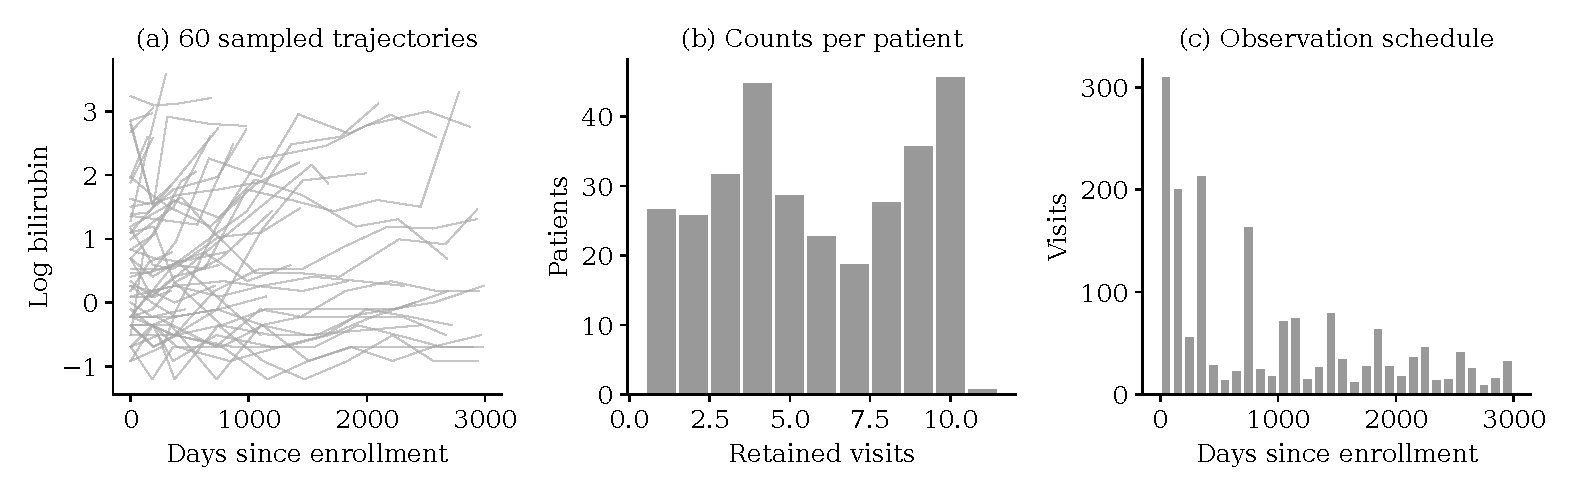
\includegraphics[width=\linewidth]{results/realdata/pbc_data_illustration.pdf}
\caption{PBC trajectories for 60 patients selected with a fixed seed, retained counts, and visit times up to day 3,000. Baseline and scheduled visits are visible.}
\label{fig:pbc-data-new}
\end{figure}

For the separate intercept-only analysis in Figure~\ref{fig:pbc-mean-new}, positive observed bilirubin and the 3,000-day restriction leave 1,790 visits from 312 patients. The equal-subject local linear estimate uses $h=0.09446$, 9,999 multipliers, and the same 201-point evaluation grid as the regression. The critical value is 2.787 and average band width is 0.555. The fit describes the weighted observed visits under the working model. Table~\ref{tab:pbc-new} summarizes the regression bandwidth sensitivity results.
\begin{figure}[!tbp]
\centering
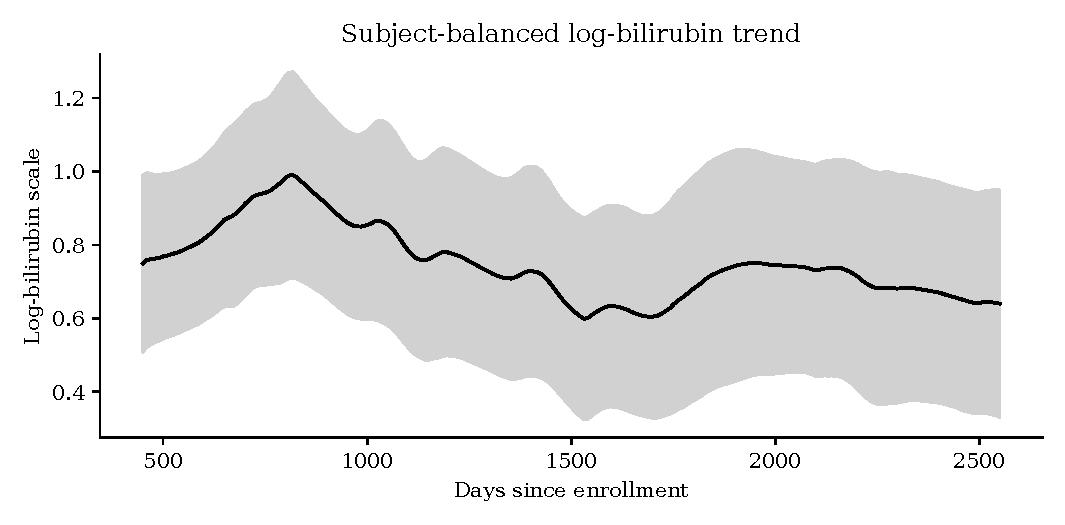
\includegraphics[width=.95\linewidth]{results/realdata/pbc_mean_bands.pdf}
\caption{Subject-balanced log-bilirubin trend and nominal 95\% band under the working sampling model.}
\label{fig:pbc-mean-new}
\end{figure}
\begin{table}[!tbp]
\centering
\caption{PBC nominal joint-band average widths for three bandwidth factors. The primary factor is $c=1$.}\label{tab:pbc-new}
\begin{tabular}{lrrr}
\toprule
Coefficient & $c=0.8$ & $c=1$ & $c=1.2$\\
\midrule
Intercept & 0.774 & 0.647 & 0.602\\
D-penicillamine & 1.056 & 0.899 & 0.846\\
Edema & 0.593 & 0.483 & 0.441\\
Albumin & 0.731 & 0.621 & 0.579\\
Prothrombin time & 0.767 & 0.670 & 0.629\\
Log ALP & 0.579 & 0.500 & 0.467\\
\bottomrule\end{tabular}\end{table}

\FloatBarrier
